\documentclass{article}
\input{/home/ishaq/preamble.tex}

\title{How do gender and smoking status influence gene expression levels?\\
\large{Testing different Hypotheses}}
\author{\LARGE{Ishaq Hamza}}
\date{22187}

\begin{document}
\maketitle

\section{Theory}
We attempt to solve the general problem of determining how the means of distributions across several \textit{feature-classes} influence (mathematically) the means of the distributions of different \textit{groups} which are realizations of comninations of the features, under an assumption of causal effects being linear.

\subsection{Formal Definitions}
\begin{definition}
    \textbf{Data} Data $\mathcal{D}$ is a set of `instances'. The formalities will be clear from context and the following definitions.
\end{definition}

\begin{definition}
    \textbf{(Features)} Features are (preferably independent) attributes assigned to each instance of a dataset. Mathematically, a feature is a pair $(\mathcal{F}, f: \mathcal{D} \to \mathcal{F})$. We shall use $f$ and $\mathcal{F}$ interchangeably.
\end{definition}
\begin{remark}
    Features are usually those attributes which arise due to natural causes, and their measurement is assumned to be flawless. In our case, the features are gender $= \{\text{male}, \text{ female}\}$ and smoking status $= \{\text{smoker}, \text{ non-smoker}\}$.
\end{remark}

\begin{definition}
    \textbf{(Feature-Class)} Given a feature $f$, and a subset $\mathcal{C} \subseteq \mathcal{F}$, the feature-class of $\mathcal{C}$ is the set of all instances that have their feature value in $\mathcal{C}$. Formally, the feature class of $\mathcal{C}$ is $f^{-1}(\mathcal{C})$
\end{definition}
\begin{remark}
    We usually use $\mathcal{C}$ and its feature class interchangeably. In our case, we will simply deal with two feature classes in each feature, namely $\{\text{males}\}, \{\text{females}\} \subseteq \text{gender}$ and $\{\text{smokers}\}, \{\text{non-smokers}\} \subseteq \text{smoking status}$.
\end{remark}

\begin{definition}
    \textbf{(Group)} A group is a set of instances sharing the same feature class, across all features. Formally, given feature-classes $\mathcal{C}_1 \subseteq{\mathcal{F}_1}, \dots, \mathcal{C}_k \subseteq \mathcal{F}_k$, group $G(\mathcal{C}_1, \dots, \mathcal{C}_k) = f_1^{-1}(\mathcal{C}_1) \cap \dots \cap f_k^{-1}(\mathcal{C}_k)$.
\end{definition}
\begin{remark}
    In our case, we will study four groups, namely $G$(male, non-smoker), $G$(male, smoker), $G$(female, non-smoker), $G$(female, smoker).
\end{remark}

\begin{definition}
    \textbf{(Observable)} An observable is a function $O: \mathcal{D} \to \mathbb{R}$ that assigns a real number to each instance.
\end{definition}
\begin{remark}
    In our case, every probe is an observable.
\end{remark}

\subsection{Hypothesis Testing: Linear Causal Model vs Independence of Groups}
Let the means of the distributions of the feature-classes be $\mu_{\mathcal{C}_1}, \dots, \mu_{\mathcal{C}_k}$, and the means of the distributions of the groups be $\mu_{G(\mathcal{C}_1, \dots, \mathcal{C}_k)}$. The \textit{Linear Causal Model} is the assumption that the means of the groups are linear combinations of the means of the feature-classes. Formally, $\mu_{G(\mathcal{C}_1, \dots, \mathcal{C}_k)} = \sum_{i=1}^k \alpha_i \mu_{\mathcal{C}_i}$.

On a fixed observable, We shall test two different hypotheses on a set of groups $\mathcal{G}$ which partition $\mathcal{D}$. The null hypthesis $H_0$: means of groups are linear causes of the means of feature-classes, and the alternative hypothesis $H_1$: the means of the groups are independent of the means of the feature-classes. Formally
\begin{align*}
    H_0 & : \mu_{G(\mathcal{C}_1, \dots, \mathcal{C}_k)} = \sum_{i=1}^k \alpha_i \mu_{\mathcal{C}_i} \ \ \forall G \in \mathcal{G} \\
    H_1 & : \mu_{G(\mathcal{C}_1, \dots, \mathcal{C}_k)} = \mu_G \in \mathbb{R}
\end{align*}
We shall define some quantities which will help us in computing the test statistic.

\begin{definition}
    \textbf{(Effect Vector)} Given a hypothesis $H: \mu_{G(\mathcal{C}_1, \dots, \mathcal{C}_k)} = \sum_{i=1}^k \alpha_i \mu_i$, the effect vector of group $G$ under hypothesis $H$ is the vector $\alpha = (\alpha_1, \dots, \alpha_k)$.
\end{definition}
\begin{remark}
    The effect vector under the alternate hypothesis of any group is a basis vector.
\end{remark}
\begin{definition}
    \textbf{(Effect Matrix)} Given a Hypothesis $H$ and a set of groups $\mathcal{G}$, the effect matrix of $\mathcal{G}$ under hypothesis $H$ is a $\abs{\mathcal{D}} \times \abs{\mathcal{G}}$ matrix whose $i$-th row is the effect vector of the group which contains the $i$-th instance, under hypothesis $H$.
\end{definition}

We shall now provide the famous two-way-anova test statistic and list a few thoerems without proof, but an intuitive explanation will be provided.

Let the effect matrix of the null hypothesis be $N$ and the effect matrix of the alternative hypothesis be $D$. Then the test statistic is
\begin{equation}
    T = \frac{\frac{1}{rD - rN} X^T (I - N(N^T N)^\dagger N^T) X}{\frac{1}{n - rD} X^T (I - D(D^T D)^\dagger D^T) X}
\end{equation}
Where $X$ is the matrix of observables, each column being an instance, $r$ is the rank operator, and $\dagger$ is the Moore-Penrose pseudoinverse.

\begin{theorem}
    Test requires rank of the effect matrix under null hypothesis $<$ rank of the effect matrix under alternative hypothesis.
\end{theorem}
\textit{Intuition.} If the effect matrix of the null hypothesis has a higher rank than the effect matrix of the alternative hypothesis, then all instances can be explained sufficiently well by the null hypothesis, leading the testing problem to be undecidable.

\section{Implementation Summary}
The data was loaded into a \texttt{pandas DataFrame} and any rows which did not have a probe name, were missing an expression level or were missing a gene symbol were dropped (we chose gene symbol as more entries had a gene symbol present).

The test described in our theory was implemented in the \texttt{anova\_two\_way} function whose pseudocode will be provided. Computation of the effect matrices for our data was covered in the lectures, hence we do avoid the details here. Some key variables and arrays are discussed below.
\begin{itemize}
    \item \texttt{observations} is a $\abs{\mathcal{D}} \times \abs{\mathcal{G}}$ matrix whose $i$-th column is the vector of observables of the $i$-th instance.
    \item \texttt{groups} is a list of indices of columns of \texttt{observations} which correspond to instances in the same group.
    \item \texttt{effect\_vectors\_null} is a $\abs{\mathcal{G}} \times \abs{\mathcal{F}}$ matrix whose $i$-th row is the effect vector of the $i$-th group under the null hypothesis.
    \item \texttt{effect\_vectors\_alternate} is a $\abs{\mathcal{G}} \times \abs{\mathcal{G}}$ matrix whose $i$-th row is the effect vector of the $i$-th group under the alternative hypothesis.
    \item \texttt{effect\_matrix\_null} and \texttt{effect\_matrix\_alternate} are the effect matrices of the null and alternative hypotheses respectively.
\end{itemize}

\begin{verbatim}
    Func h_test

    Require: observations, groups, effect_vectors_null, effect_vectors_alternate

    Output: array of p-values
             array[i] = p_value of the test for the i-th observable

    compute the effect matrices, their ranks and dimensions

    numerators = [observations[i](I-N(N* N)dagger N*)observations[i]* |i in [num_observations]]

    denominators = [observations[i](I-D(D* D)dagger D*)observations[i]* |i in [num_observations]]

    ratios = [numerator[i] / denominator[i] | i in [num_observations]]  // zero division handled

    Output [1 - F.cdf(deg_freedom_numerator, deg_freedom_denominator)(ratio) | ratio in ratios]
\end{verbatim}

Where we handled zero division by the function \texttt{smart\_ratio} which takes $0/0 = 1$, $x/0 = \infty$ for positive $x$.

For computing \texttt{numerator} and \texttt{denominator}, we used the Einstein summation convention, which is implemented in the \texttt{einsum} function in \texttt{numpy}. The usage of \texttt{np.einsum('ij,jk,ki->i', A, B, C)} is equivalent to computing the diagonal elements in the product $ABC$.

We did not obtain a uniform distribution of p-values (which should be expected from the reasons we describe shortly). We suspected that multiple probes measuring expression levels of the same gene could cause repeated data, and hence we chose to aggregate by three methods (mean, median, max) and plotted p-values for the same.

\section{Code Output and Conclusions}
\texttt{Removed 9072 rows with missing values}\\
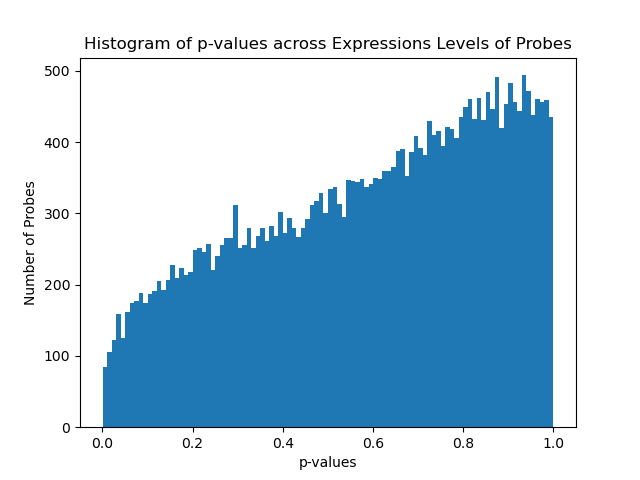
\includegraphics{Plot1.png}\\
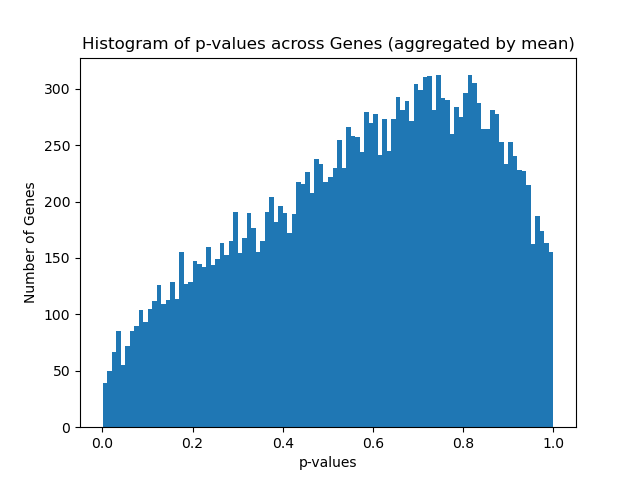
\includegraphics{Plot2.png}\\
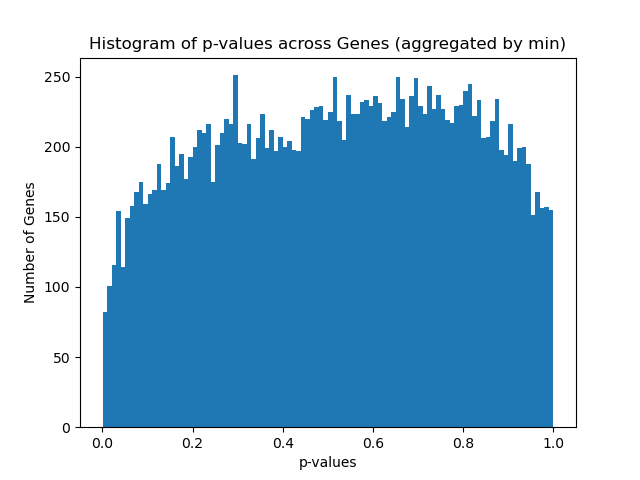
\includegraphics{Plot3.png}\\
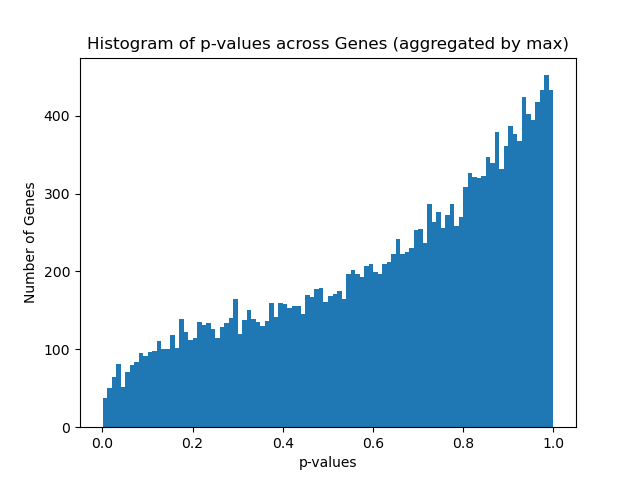
\includegraphics{Plot4.png}\\
We would expect a uniform distributions of p-values, but that is not the case here, there are more gene-expressions whose p-values are high. This can be explained due the following reasons:
\begin{itemize}
    \item The data underlying data is not not normally distributed, as we would express gene expressions to be non-negative.
    \item data tranformation was done (max(0, $\log$(gene expression))) was used, this neglects all values smaller than 1. And changes the underlying distribution as well.
    \item multiple probes corresponding to the same gene might have correlation.
\end{itemize}
We shall examine the suspicion that multiple probes corresponding to the same gene might have correlation. We aggregated different probes corresponding to the same gene by three methods (mean, min, max). If our claim is correct, then the p-values aggregated by mean should have a distribution closer to uniform.

From the plots, we found that the distribution is closer to uniform, but there is a shift of peak from 0.9 to 0.7 which we could not explain. Since our claim is correct, we explored a few more aggregates (min and max). With the suspicion being that min would have a distribution closer to uniform, and max would make it worse. The plots confirmed our suspicion. However, these are hacks and not a proper solution as the main probelm is due to lack of normality in the data itself.

In order to truly fix the non-uniform p-values issue, one could use the famous box-cox tranformation on the original data instead of the transformation used here. But any form of data manipulation introduces bias and effects variance, hence any hypothesis test on transformed data could be misleadingly good/bad. One should rather use tests which do not assume normality of the data, such as the Wilcoxon rank-sum test.
\end{document}